% Provenance (never printed): see sources/outline_sources.md (Year 3:
% geophysical fluid dynamics: rotating-frame equations, Rossby number,
% hydrostatic and geostrophic balance, thermal wind, buoyancy frequency).
% Brief: sources/book5/BRIEFS.md, ch. 19. Curves from
% figdata/bachelor-3/inertial_oscillation.py, thermal_wind.py and
% buoyancy_frequency.py. Exercise and problem values in the Book 5 scratch
% calculator calc/ch19.py. The Steppe of Orrin, its lake, its stations and
% its winds are invented.
\chapter{Geophysical Fluid Dynamics}\label{ch:b3:gfd-foundations}

Stir a cup of tea and the swirl dies in a minute; the leaves gather in the
middle of the bottom and nothing else happens. The ocean and the atmosphere
are stirred too, by the Sun and the wind, but on a rotating planet and in
layers of different density. Rotation and stratification make them obey
rules that a teacup never shows: winds blow along the isobars instead of
across them, columns of fluid refuse to tilt, and the wind of the upper
troposphere is written in the temperatures below it. This chapter sets up
the equations of these large, slow, thin flows and the few numbers that
decide which terms matter.

\begin{recall}
The Coriolis and centrifugal forces in a rotating frame, the Navier--Stokes
and continuity equations, viscosity, the Reynolds number and the hydrostatic
relation are in the physics books. The Coriolis parameter $f = 2\Omega
\sin\varphi$, the pressure-gradient force, geostrophic balance, the
geostrophic and \omterm{def:b3:gfd-foundations:gradient}{gradient winds} and the jet streams are in the Year~1
volume, in its chapter on the general circulation of the atmosphere; the
Ekman layer in its chapter on the circulation of the ocean; potential
temperature, static stability and the oscillation of a lifted air parcel in
its chapter on the structure of the atmosphere and the ocean.
\end{recall}

\section{Equations in a rotating frame}\label{sec:b3:gfd-foundations:equations}

In a frame that turns with the Earth at the angular velocity
$\vec\Omega$, a fluid parcel of velocity $\vec u$ obeys
\[
\frac{\mathrm D\vec u}{\mathrm Dt} + 2\vec\Omega\times\vec u =
-\frac{1}{\rho}\nabla p + \vec g + \nu\nabla^2\vec u ,
\qquad
\frac{\partial\rho}{\partial t} + \nabla\cdot(\rho\vec u) = 0 ,
\]
where $\mathrm D/\mathrm Dt = \partial/\partial t + \vec u\cdot\nabla$ is
the derivative following the parcel and $\nu$ the kinematic viscosity. The
centrifugal force has been added to gravitation: their sum $\vec g$ is the
effective gravity, normal to the level surfaces of the \omterm{def:b3:gravity-geodesy:geopotential}{geopotential}, and
the vertical is defined by it. Only the Coriolis term, $-2\vec\Omega\times
\vec u$, remains of the rotation, and it does no work: it turns a parcel
without changing its speed. The Earth turns at $\Omega =
\qty{7.292115e-5}{rad/s}$, once a sidereal day of \qty{23.9345}{h}.
% ledger: geod5:grs80-defining, earth:Trot

For motion over distances much smaller than the Earth's radius $a$, a
local Cartesian frame is enough: $x$ eastward, $y$ northward, $z$ upward,
at the latitude $\varphi$, the tangent plane of the figure below. There
$\vec\Omega = \Omega\,(0, \cos\varphi, \sin\varphi)$, and the three
components of the momentum equation are
\[
\begin{aligned}
\frac{\mathrm Du}{\mathrm Dt} - f v + \tilde f w &= -\frac{1}{\rho}\frac{\partial p}{\partial x} + F_x ,\\
\frac{\mathrm Dv}{\mathrm Dt} + f u &= -\frac{1}{\rho}\frac{\partial p}{\partial y} + F_y ,\\
\frac{\mathrm Dw}{\mathrm Dt} - \tilde f u &= -\frac{1}{\rho}\frac{\partial p}{\partial z} - g + F_z ,
\end{aligned}
\qquad f = 2\Omega\sin\varphi,\quad \tilde f = 2\Omega\cos\varphi ,
\]
with $\vec F$ the friction. For the thin, nearly horizontal flows of the
ocean and the atmosphere the terms in $\tilde f$ are dropped: $\tilde f w$
is small beside $fv$ because $w \ll v$, and $\tilde f u$ is a ten-thousandth
of $g$ (\cref{exo:b3:gfd-foundations:5}). The Coriolis force then acts only
in the horizontal, through the local vertical component of the rotation,
$\Omega\sin\varphi$.

\begin{definition}[$f$-plane and $\beta$-plane]\label{def:b3:gfd-foundations:planes}
Near a reference latitude $\varphi_0$, the \emph{$f$-plane}\index{f-plane@$f$-plane}
approximation takes the Coriolis parameter as constant, $f = f_0 =
2\Omega\sin\varphi_0$. The \emph{$\beta$-plane}\index{beta-plane@$\beta$-plane}
approximation keeps its first-order change with the northward distance $y$:
$f = f_0 + \beta y$, with $\beta = \mathrm df/\mathrm dy = 2\Omega
\cos\varphi_0/a$.
\end{definition}

At \ang{45}, with the mean radius $a = \qty{6371}{km}$, $f_0 =
\qty{1.031e-4}{s^{-1}}$ and $\beta = \qty{1.62e-11}{m^{-1}.s^{-1}}$: over
\qty{1000}{km} of latitude $f$ changes by \qty{16}{\percent}. The $f$-plane
suits motions much smaller than that; the $\beta$-plane is needed for
basin-wide currents and planetary waves.
% ledger: earth:Rmean, geod5:grs80-defining (values in figdata/bachelor-3/inertial_oscillation.py)

\begin{omfigure}
\begin{minipage}[c]{0.42\linewidth}\centering
\begin{tikzpicture}[>=stealth, font=\small]
\draw[thick] (0,0) circle (2);
\draw[black!40, dashed] (-2,0) -- (2,0);
\draw[->, thick] (0,-2.4) -- (0,2.75) node[above] {$\vec\Omega$};
\draw (0,0) -- (30:2) coordinate (P);
\draw (0.6,0) arc (0:30:0.6);
\node at (15:0.9) {$\varphi$};
\draw[black!60] ($(P)+(120:-1.1)$) -- ($(P)+(120:1.3)$);
\draw[->, omThm, thick] (P) -- ++(0,1.6) node[right] {$\vec\Omega$};
\draw[->, omDef, thick] (P) -- ++(30:0.8) node[anchor=south west, align=left, inner sep=1pt] {$\Omega\sin\varphi$,\\ up};
\draw[->, omMeth, thick] (P) -- ++(120:1.386) node[anchor=south, align=center, inner sep=1pt] {$\Omega\cos\varphi$,\\ north};
\draw[black!50, densely dotted] ($(P)+(30:0.8)$) -- ($(P)+(0,1.6)$) -- ($(P)+(120:1.386)$);
\draw (P) circle (0.09); \draw ($(P)+(-0.064,-0.064)$) -- ($(P)+(0.064,0.064)$);
\draw ($(P)+(-0.064,0.064)$) -- ($(P)+(0.064,-0.064)$);
\node[font=\scriptsize, anchor=west] at ($(P)+(0.14,-0.03)$) {$x$, east};
\node[font=\scriptsize, black!60] at (-1.15,-0.25) {equator};
\end{tikzpicture}
\end{minipage}\hfill
\begin{minipage}[c]{0.55\linewidth}\centering
\begin{tikzpicture}
\begin{axis}[width=\linewidth, height=0.72\linewidth, xmin=0, xmax=90, ymin=0, ymax=1.8,
  xlabel={latitude (\unit{\degree})}, ylabel={$f$ ($10^{-4}$\,\unit{s^{-1}})},
  xtick={0,15,30,45,60,75,90}, tick label style={font=\scriptsize}, label style={font=\small},
  legend style={font=\scriptsize, draw=none, fill=none}, legend pos=north west]
% computed in figdata/bachelor-3/inertial_oscillation.py
\addplot[omDef, thick] table[x=lat, y=f] {figdata/out/bachelor-3-inertial_oscillation-fbeta.dat};
\addplot[omThm, densely dashed] table[x=lat, y=fb] {figdata/out/bachelor-3-inertial_oscillation-fbeta.dat};
\addplot[only marks, mark=*, mark size=1.6pt] coordinates {(45,1.03126)};
\legend{$2\Omega\sin\varphi$, $\beta$-plane at \ang{45}}
\end{axis}
\end{tikzpicture}
\end{minipage}

\par\smallskip{\small Left, the local frame at latitude $\varphi$: $z$
along the local vertical, $y$ northward in the tangent plane, $x$ eastward
into the page. The rotation vector splits into $\Omega\sin\varphi$ about the
vertical, which turns horizontal motion, and $\Omega\cos\varphi$ about the
northward axis, dropped for thin flows. Right, the Coriolis parameter and
its $\beta$-plane tangent at \ang{45}: close over a band of latitude, far
from it near the equator and the pole.}\label{fig:b3:gfd-foundations:frame}
\end{omfigure}
% ledger: geod5:grs80-defining, earth:Rmean

Two more approximations simplify the equations without losing what
matters. The first concerns density.

\begin{definition}[Boussinesq approximation]\label{def:b3:gfd-foundations:boussinesq}
The \emph{Boussinesq approximation}\index{Boussinesq approximation} writes
the density as $\rho = \rho_0 + \rho'$, with $\rho_0$ a constant and
$|\rho'| \ll \rho_0$, and keeps $\rho'$ only where it is multiplied by $g$.
The continuity equation becomes $\nabla\cdot\vec u = 0$, and the momentum
equation
\[
\frac{\mathrm D\vec u}{\mathrm Dt} + f\,\vec k\times\vec u =
-\frac{1}{\rho_0}\nabla p' + b\,\vec k + \nu\nabla^2\vec u ,
\qquad b = -g\,\frac{\rho'}{\rho_0} ,
\]
where $p'$ is the departure of the pressure from the hydrostatic pressure
of the density $\rho_0$, $\vec k$ the upward unit vector and $b$ the
buoyancy.
\end{definition}

In the ocean $\rho'$ is a few \unit{kg/m^3} on \num{1025}, a fraction of a
per cent, and the approximation is excellent. In the atmosphere density
falls by a factor $e$ in about \qty{8.5}{km}; the approximation holds for
layers much thinner than that, and deeper flows replace $\rho_0$ by a
mean profile $\rho_0(z)$, with the same physics.
% ledger: earth:Hscale

The second concerns the vertical. A fluid at rest is in hydrostatic
equilibrium; a fluid in motion keeps it to a very good approximation when
the motion is much wider than it is deep.

\begin{definition}[Hydrostatic approximation]\label{def:b3:gfd-foundations:hydrostatic}
The \emph{hydrostatic approximation}\index{hydrostatic approximation}
replaces the vertical momentum equation of a moving fluid by the
hydrostatic relation, $\partial p/\partial z = -\rho g$.
\end{definition}

\begin{proposition}[When the hydrostatic approximation holds]\label{prop:b3:gfd-foundations:hydrostatic}
For a motion of horizontal scale $L$, depth $H$ and speed $U$, with a
\omterm{def:b3:gfd-foundations:numbers}{Rossby number} $U/(fL)$ at most of order one, the vertical acceleration is
smaller than the vertical gradient of the pressure perturbation by a factor
of order $(U/fL)\,(H/L)^2$.
\end{proposition}

\begin{proof}
When the Coriolis force is at least as large as the acceleration, the
horizontal momentum equation balances the horizontal pressure gradient
against it: $p'/(\rho_0 L) \sim fU$, so $p'/\rho_0 \sim fUL$, and the vertical
gradient is $p'/(\rho_0 H) \sim fUL/H$. Continuity, $\partial w/\partial z
= -(\partial u/\partial x + \partial v/\partial y)$, bounds the vertical
velocity by $W \sim UH/L$, and the vertical acceleration by
$\mathrm Dw/\mathrm Dt \sim UW/L = U^2H/L^2$. The ratio is $(U^2H/L^2)/(fUL/H)
= (U/fL)(H/L)^2$.
\end{proof}

A weather system \qty{1000}{km} wide in a troposphere \qty{10}{km} deep has
$(H/L)^2 = 10^{-4}$ and a \omterm{def:b3:gfd-foundations:numbers}{Rossby number} of about 0.1: the error of the
\omterm{def:b3:gfd-foundations:hydrostatic}{hydrostatic approximation} is of order $10^{-5}$. It fails only in narrow, deep motions: a
thunderstorm updraught, a convective plume in the ocean.

\section{Scales of rotating flow}\label{sec:b3:gfd-foundations:scales}

Which terms of the momentum equation matter is decided by two ratios.

\begin{definition}[Rossby and Ekman numbers]\label{def:b3:gfd-foundations:numbers}
For a flow of speed $U$, horizontal scale $L$ and depth $H$ on a planet of
Coriolis parameter $f$, the \emph{Rossby number}\index{Rossby number} is
$\mathrm{Ro} = U/(fL)$, the ratio of the acceleration, of order $U^2/L$,
to the Coriolis force, of order $fU$. The \emph{Ekman
number}\index{Ekman number} is $\mathrm{Ek} = \nu/(fH^2)$, the ratio of
the viscous force, of order $\nu U/H^2$, to the Coriolis force; in a
turbulent flow $\nu$ is replaced by an eddy viscosity.
\end{definition}

A bathtub draining \qty{0.1}{m/s} over \qty{0.3}{m} has a \omterm{def:b3:gfd-foundations:numbers}{Rossby number} of
some thousands: the Earth's rotation does not decide the sense of its
swirl. A depression \qty{1000}{km} across with winds of \qty{15}{m/s} has
$\mathrm{Ro} \approx 0.14$, and an ocean gyre $\mathrm{Ro} \sim 10^{-4}$.
Viscosity is weaker still: the molecular viscosity of water is
\qty{e-6}{m^2/s}, and the eddy viscosities that stand for the turbulence
of the ocean, \qtyrange{e-5}{e-3}{m^2/s} in the vertical, give
$\mathrm{Ek} \sim 10^{-5}$ over \qty{1000}{m} of depth. The two numbers are
related to the Reynolds number by $\mathrm{Re} = UL/\nu =
(\mathrm{Ro}/\mathrm{Ek})(L/H)^2$.
% ledger: stewart:eddy (problem values in calc/ch19.py)

When both numbers are small, the steady horizontal momentum equation keeps
only the Coriolis force and the pressure gradient: the flow is in
geostrophic balance, $f\,\vec k\times\vec u_g = -(1/\rho)\nabla_h p$, which
the Year~1 volume read from weather maps. Geostrophy is the limit
$\mathrm{Ro}, \mathrm{Ek}\to 0$; its corrections are of order
$\mathrm{Ro}$, and friction acts only in thin layers of relative thickness
$\sqrt{\mathrm{Ek}}$, the Ekman layers at the bottom of the atmosphere and
the top and bottom of the ocean. On an $f$-plane the geostrophic velocity
has no horizontal divergence: $\partial u_g/\partial x + \partial
v_g/\partial y = -(1/\rho f)(\partial^2 p/\partial x\partial y -
\partial^2 p/\partial y\partial x) = 0$ for uniform $\rho$.

The opposite limit, rotation with no pressure gradient, is the simplest
motion a rotating fluid can make.

\begin{definition}[Inertial oscillation]\label{def:b3:gfd-foundations:inertial}
An \emph{inertial oscillation}\index{inertial oscillation} is the
horizontal motion of a fluid on which no horizontal force acts but the
Coriolis force.
\end{definition}

\begin{theorem}[Inertial circles]\label{thm:b3:gfd-foundations:inertial}
On an $f$-plane, a parcel set moving at speed $U$ with no horizontal force
but the Coriolis force keeps its speed and describes a circle of radius
$U/|f|$, clockwise in the Northern Hemisphere and anticlockwise in the
Southern, in the inertial period $2\pi/|f|$, which is half a sidereal day
divided by $\sin\varphi$.
\end{theorem}

\begin{proof}
The equations are $\mathrm du/\mathrm dt = fv$, $\mathrm dv/\mathrm dt =
-fu$. With $w = u + \mathrm iv$ they read $\mathrm dw/\mathrm dt = -\mathrm
if\,w$, so $w = U\,\mathrm e^{-\mathrm ift}$ for a start eastward: the
speed $|w| = U$ is constant and the velocity turns at the rate $f$,
clockwise when $f > 0$. Integrating, the position $x + \mathrm iy =
(\mathrm iU/f)(\mathrm e^{-\mathrm ift} - 1)$ runs round the point
$-\mathrm iU/f$ at the distance $U/|f|$. The period is $2\pi/|f| =
2\pi/(2\Omega|\sin\varphi|)$, and $2\pi/\Omega$ is the sidereal day.
\end{proof}

At \ang{45} the inertial period is \qty{16.9}{h}, and a current of
\qty{0.2}{m/s} turns on a circle of \qty{1.94}{km}; at \ang{30} the period
is a full sidereal day, and at the equator there are no inertial circles.
After a storm has set the surface layer of the ocean moving and then died,
the water does exactly this. Drogued drifting buoys at \qty{15}{m} in the
North Pacific traced loops for days after a storm in October 1987, carried
along by the mean current: the third path of the figure below, after the
circle and the spiral.
% ledger: stewart:inertial, earth:Trot (values in figdata/bachelor-3/inertial_oscillation.py)

\begin{omfigure}
\begin{tikzpicture}
\begin{axis}[width=\linewidth, axis equal image, xmin=-3, xmax=18.5, ymin=-4.6, ymax=1.2,
  xlabel={eastward distance (km)}, ylabel={northward (km)},
  tick label style={font=\scriptsize}, label style={font=\small},
  legend style={font=\scriptsize, draw=none, fill=white, fill opacity=0.85, text opacity=1},
  legend pos=south east, legend columns=3]
% computed in figdata/bachelor-3/inertial_oscillation.py
\addplot[black!45, line width=1.6pt] table[x=x, y=y] {figdata/out/bachelor-3-inertial_oscillation-circle.dat};
\addplot[omDef, thick] table[x=x, y=y] {figdata/out/bachelor-3-inertial_oscillation-spiral.dat};
\addplot[omThm, thick] table[x=x, y=y] {figdata/out/bachelor-3-inertial_oscillation-loops.dat};
\addplot[only marks, mark=*, mark size=1.8pt] coordinates {(0,0)};
\legend{no friction, friction, friction and current}
\end{axis}
\end{tikzpicture}

\par\smallskip{\small Paths over four days of a parcel set moving
eastward at \qty{0.2}{m/s} at \ang{45} N (dot), with no force but the
Coriolis force: a circle of radius \qty{1.94}{km} run clockwise every
\qty{16.9}{h} (grey); with a friction that halves the speed in
\num{2.8}~days, an inward spiral (blue); the same carried by a steady
eastward current of \qty{0.05}{m/s}, a train of shrinking loops
(red).}\label{fig:b3:gfd-foundations:inertial}
\end{omfigure}
% ledger: stewart:inertial

Between geostrophy and the inertial circle lies the flow round a centre of
high or low pressure, where the isobars are curved and the acceleration
towards the centre is no longer negligible.

\begin{definition}[Gradient wind]\label{def:b3:gfd-foundations:gradient}
The \emph{gradient wind}\index{gradient wind} is the steady, frictionless
flow along curved isobars in which the pressure-gradient force, the
Coriolis force and the centripetal acceleration balance.
\end{definition}

\begin{proposition}[The curvature correction]\label{prop:b3:gfd-foundations:gradient}
Let the isobars be circles of radius $r$ in the Northern Hemisphere, and
$V_g$ the geostrophic speed that their pressure gradient would give, with
$\mathrm{Ro}_g = V_g/(fr)$. Round a low, the \omterm{def:b3:gfd-foundations:gradient}{gradient wind} is
$V = 2V_g/(1 + \sqrt{1 + 4\mathrm{Ro}_g})$, slower than $V_g$; round a
high, $V = 2V_g/(1 + \sqrt{1 - 4\mathrm{Ro}_g})$, faster, and it exists only
if $\mathrm{Ro}_g \le 1/4$. To first order, $V = V_g(1 \mp \mathrm{Ro}_g)$.
\end{proposition}

\begin{proof}
Round a low the wind turns anticlockwise; the pressure-gradient force
$fV_g$ points to the centre, the Coriolis force $fV$ outward, and their
difference provides the centripetal acceleration: $fV_g - fV = V^2/r$. The
positive root of $V^2 + frV - frV_g = 0$ is $V = (fr/2)(\sqrt{1 +
4\mathrm{Ro}_g} - 1)$; multiplying by $(\sqrt{1 + 4\mathrm{Ro}_g} +
1)/(\sqrt{1 + 4\mathrm{Ro}_g} + 1)$ gives the formula. Round a high, the
wind turns clockwise and the Coriolis force points inward: $fV - fV_g =
V^2/r$, so $V^2 - frV + frV_g = 0$, which has real roots only if $f^2r^2
\ge 4frV_g$; the root that tends to $V_g$ when $\mathrm{Ro}_g \to 0$ is
$V = (fr/2)(1 - \sqrt{1 - 4\mathrm{Ro}_g})$. Expanding the square roots,
$V = V_g(1 \mp \mathrm{Ro}_g + \dots)$.
\end{proof}

The \omterm{def:b3:gfd-foundations:numbers}{Rossby number} of the isobars measures the correction: a tenth for a
depression of moderate size. The condition $\mathrm{Ro}_g \le 1/4$ is why
the centre of an anticyclone has weak gradients and light winds, while
that of a depression can hold steep gradients and gales.

\section{Rotation without stratification}\label{sec:b3:gfd-foundations:taylor}

A rotating fluid of uniform density, in slow motion, behaves as if it were
made of rigid columns parallel to the rotation axis.

\begin{theorem}[Taylor--Proudman]\label{thm:b3:gfd-foundations:taylor-proudman}
In a steady flow of an inviscid fluid of uniform density, rotating at
$\vec\Omega$, with small \omterm{def:b3:gfd-foundations:numbers}{Rossby number}, the velocity does not vary along
the direction of the rotation axis: $(\vec\Omega\cdot\nabla)\vec u = 0$.
\end{theorem}
\index{Taylor--Proudman theorem}

\begin{proof}
For $\mathrm{Ro}\to 0$, steady and inviscid, the momentum equation reduces
to $2\vec\Omega\times\vec u = -\nabla(p/\rho_0 + \Phi)$, with $\Phi$ the
\omterm{def:b3:gravity-geodesy:geopotential}{geopotential}. The curl of a gradient vanishes, so $\nabla\times(\vec\Omega
\times\vec u) = 0$. For a constant $\vec\Omega$ this curl is $\vec\Omega
(\nabla\cdot\vec u) - (\vec\Omega\cdot\nabla)\vec u$, and $\nabla\cdot\vec u
= 0$ for uniform density.
\end{proof}

With $\vec\Omega$ along $z$, $\partial\vec u/\partial z = 0$: all three
velocity components are the same at every height. If a rigid bottom forbids
$w$ there, $w = 0$ everywhere, and the horizontal flow is the same at every
level. An obstacle on the floor of a rotating tank is therefore felt all
the way to the surface: the fluid above it cannot climb over it, since
that would stretch or squeeze a column, and goes round it at every height.
The column of fluid that stays above the obstacle is a \emph{Taylor
column}\index{Taylor column}.

\begin{omfigure}
\begin{tikzpicture}[>=stealth, font=\small]
% side view
\fill[omDef!8] (0,0) rectangle (5.4,3);
\fill[black!10] (2.1,0) rectangle (3.3,3);
\draw[thick] (0,3.3) -- (0,0) -- (5.4,0) -- (5.4,3.3);
\draw[black!50] (0,3) -- (5.4,3);
\draw[fill=black!45] (2.1,0) .. controls (2.4,0.55) and (3.0,0.55) .. (3.3,0) -- cycle;
\draw[black!60, densely dashed] (2.1,0) -- (2.1,3) (3.3,0) -- (3.3,3);
\foreach \y in {0.8,1.6,2.4} {\draw[->, omDef, thick] (0.3,\y) -- (1.9,\y);
  \draw[->, omDef, thick] (3.5,\y) -- (5.1,\y);}
\draw[->, thick, omThm] (2.7,3.25) -- (2.7,4.0) node[right] {$\vec\Omega$};
\node[font=\scriptsize, align=center] at (2.7,1.7) {Taylor\\column};
\node[font=\scriptsize, anchor=north] at (2.7,-0.05) {obstacle};
\node[font=\small] at (2.7,-0.6) {(a) side view};
% top view
\begin{scope}[xshift=6.4cm]
\fill[omDef!8] (0,0) rectangle (5.4,3);
\draw[thick] (0,0) rectangle (5.4,3);
\fill[black!10] (2.7,1.5) circle (0.5);
\draw[black!60, densely dashed] (2.7,1.5) circle (0.5);
\foreach \d/\h in {0.3/0.10, 0.75/0.35, 1.2/0.58} {
  \draw[->, omDef, thick] (0.2,1.5+\d) .. controls (1.6,1.5+\d) and (2.0,1.5+\h+0.62) .. (2.7,1.5+\h+0.62)
     .. controls (3.4,1.5+\h+0.62) and (3.8,1.5+\d) .. (5.2,1.5+\d);
  \draw[->, omDef, thick] (0.2,1.5-\d) .. controls (1.6,1.5-\d) and (2.0,1.5-\h-0.62) .. (2.7,1.5-\h-0.62)
     .. controls (3.4,1.5-\h-0.62) and (3.8,1.5-\d) .. (5.2,1.5-\d);}
\node[font=\small] at (2.7,-0.6) {(b) seen from above, at any height};
\end{scope}
\end{tikzpicture}

\par\smallskip{\small A \omterm{thm:b3:gfd-foundations:taylor-proudman}{Taylor column} (schematic). (a) In a tank of
uniform water rotating rapidly, a slow flow meets a low obstacle on the
floor; the fluid above the obstacle (grey) is held in place up to the
surface, and the flow at every height goes round the column as if the
obstacle reached the top. (b) The flow seen from above is the same at
every level.}\label{fig:b3:gfd-foundations:taylor}
\end{omfigure}

The atmosphere and the ocean are stratified, and stratification relaxes
the constraint: a stratified fluid can vary with height, in the way the
\omterm{thm:b3:gfd-foundations:thermal-wind}{thermal wind} theorem prescribes.

\section{Stratification and the thermal wind}\label{sec:b3:gfd-foundations:stratification}

The Year~1 volume lifted an air parcel in a stable atmosphere and found
that it oscillates about its level. The same holds in any stratified fluid,
and the frequency of the oscillation is the measure of stratification.

\begin{definition}[Buoyancy frequency]\label{def:b3:gfd-foundations:buoyancy}
The \emph{buoyancy frequency}\index{buoyancy frequency} $N$ of a fluid at
rest is defined by
\[
N^2 = \frac{g}{\theta}\frac{\mathrm d\theta}{\mathrm dz}\ \text{(air)},
\qquad
N^2 = -\frac{g}{\rho_0}\frac{\mathrm d\rho_\theta}{\mathrm dz}\ \text{(seawater)},
\]
where $\theta$ is the potential temperature of the air and $\rho_\theta$ the
potential density of the water, the density it would have if brought
adiabatically to a reference pressure.
\end{definition}

\begin{theorem}[Oscillation of a displaced parcel]\label{thm:b3:gfd-foundations:buoyancy}
A parcel displaced vertically by a small distance $\zeta$ from its level in a
fluid at rest, adiabatically and without mixing, obeys $\ddot\zeta =
-N^2\zeta$. If $N^2 > 0$ it oscillates at the angular frequency $N$; if
$N^2 < 0$ the displacement grows and the fluid is unstable.
\end{theorem}

\begin{proof}
Moved adiabatically and without mixing, the parcel keeps its potential
density $\rho_\theta(z_0)$. At the level $z_0 + \zeta$ it is at the pressure
of its surroundings, whose potential density is $\rho_\theta(z_0) +
\zeta\,\mathrm d\rho_\theta/\mathrm dz$; two parcels at the same pressure
differ in density by the difference of their potential densities, to first
order. The buoyancy force per unit mass is $-g(\rho_p - \rho_e)/\rho_0 =
g\,\zeta\,(\mathrm d\rho_\theta/\mathrm dz)/\rho_0 = -N^2\zeta$. For air at a
given pressure the density varies as $1/\theta$, so $-\mathrm
d\rho_\theta/\rho_0 = \mathrm d\theta/\theta$ and the two forms of $N^2$
agree.
\end{proof}

In the troposphere of the standard atmosphere, which cools by
\qty{6.49}{K/km} against the \qty{9.77}{K/km} of the dry adiabat ($g/c_p$,
with $c_p = \gamma R/(\gamma - 1)$, $\gamma = 1.4$ and $R =
\qty{286.9}{J.kg^{-1}.K^{-1}}$), $N$ averages \qty{0.0113}{s^{-1}}, a period
of \qty{9.3}{min}; in the isothermal lower stratosphere it is
\qty{0.0210}{s^{-1}}. In the ocean, the water column of the North Atlantic
at \ang{40.5} N, \ang{30.5} W in the annual mean has its strongest
stratification in the seasonal pycnocline, $N = \qty{0.0106}{s^{-1}}$ at
about \qty{30}{m}, six cycles per hour, and much weaker values below: a few
cycles per hour at most, as observed across the upper ocean.
% ledger: nasa:grc-atmos, nasa:grc-gamma-b5, nws:dalr, data:b5-woa23-atlantic, unesco44:eos80-b5, stewart:stability (values in figdata/bachelor-3/buoyancy_frequency.py)

\begin{omfigure}
\begin{tikzpicture}
\begin{groupplot}[group style={group size=2 by 1, horizontal sep=1.7cm},
  width=0.48\linewidth, height=0.50\linewidth, tick label style={font=\scriptsize},
  label style={font=\small}]
\nextgroupplot[xlabel={$N$ ($10^{-2}$\,\unit{s^{-1}})}, ylabel={height (km)},
  xmin=0, xmax=3, ymin=0, ymax=30, title={\small atmosphere}]
% computed in figdata/bachelor-3/buoyancy_frequency.py
\addplot[omDef, thick] table[x expr=\thisrow{N}*100, y=z] {figdata/out/bachelor-3-buoyancy_frequency-atm.dat};
\addplot[black!50, densely dashed, domain=0:3, samples=2] {11};
\node[font=\scriptsize, anchor=south east] at (axis cs:2.95,11) {tropopause};
\nextgroupplot[xlabel={$N$ (cycles per hour)}, ylabel={depth (m)}, y dir=reverse,
  xmin=0, xmax=7, ymin=0, ymax=2000, title={\small ocean, \ang{40.5} N \ang{30.5} W},
  scaled y ticks=false, ytick={0,500,1000,1500,2000}, yticklabels={0,500,1000,1500,2000}]
\addplot[omThm, thick, mark=*, mark size=0.9pt] table[x=cph, y=z] {figdata/out/bachelor-3-buoyancy_frequency-ocean.dat};
\end{groupplot}
\end{tikzpicture}

\par\smallskip{\small \omterm{def:b3:gfd-foundations:buoyancy}{Buoyancy frequency}. Left, the standard atmosphere:
nearly uniform in the troposphere, twice as large in the isothermal lower
stratosphere, larger still above \qty{25}{km} where the temperature rises.
Right, an annual-mean column of the North Atlantic (temperature and
salinity from the World Ocean Atlas 2023, potential density from EOS-80):
a sharp maximum in the seasonal pycnocline, weak stratification
below.}\label{fig:b3:gfd-foundations:buoyancy}
\end{omfigure}
% ledger: nasa:grc-atmos, data:b5-woa23-atlantic, unesco44:eos80-b5

Stratification lets the flow vary with height, and how it does so depends
on whether the surfaces of constant density follow those of constant
pressure.

\begin{definition}[Barotropic and baroclinic fluids]\label{def:b3:gfd-foundations:baroclinic}
A fluid is \emph{barotropic}\index{barotropic fluid} if its density is a
function of pressure alone, so that surfaces of constant density coincide
with surfaces of constant pressure; it is
\emph{baroclinic}\index{baroclinic fluid} if they cross.
\end{definition}

In the atmosphere, a horizontal gradient of temperature along a pressure
surface makes the air \omterm{def:b3:gfd-foundations:baroclinic}{baroclinic}. Hydrostatic balance then makes the
pressure surfaces slope more steeply with height, and geostrophic balance
turns the growing slope into a growing wind.

\begin{omfigure}
\begin{tikzpicture}[>=stealth, font=\small, x=1.15cm, y=0.85cm]
\shade[left color=omThm!22, right color=omDef!22] (0,0) rectangle (8,4);
\draw[thick] (0,0) -- (8,0);
\foreach \k/\lab in {1/p_1, 2/p_2, 3/p_3, 4/p_4} {
  \draw[black, thick] (0,0.9*\k) -- (8,0.675*\k) node[right] {$\lab$};}
\foreach \k/\r in {1/0.07, 2/0.11, 3/0.15, 4/0.19} {
  \draw[omMeth, thick, fill=white] (4,0.7875*\k) circle (\r);
  \fill[omMeth] (4,0.7875*\k) circle (0.035);}
\node[font=\scriptsize, anchor=south west] at (4.12,3.3) {$u_g$};
\node[font=\scriptsize] at (0.8,3.8) {warm};
\node[font=\scriptsize] at (7.2,3.8) {cold};
\draw[->] (0.3,-0.35) -- (2.0,-0.35) node[right, font=\scriptsize] {north, $y$};
\end{tikzpicture}

\par\smallskip{\small The geometry of the \omterm{thm:b3:gfd-foundations:thermal-wind}{thermal wind} (schematic, a
meridional section with the warm side to the south, $p_1 > p_2 > p_3 >
p_4$). Warm air expands, so the layer between two pressure surfaces is
thicker on the warm side than on the cold: each surface slopes down
towards the cold side more steeply than the one below. The geostrophic
wind is proportional to the slope, and grows with height (circles, larger
for stronger wind), eastward, out of the
page.}\label{fig:b3:gfd-foundations:geometry}
\end{omfigure}

\begin{theorem}[Thermal wind]\label{thm:b3:gfd-foundations:thermal-wind}
In an atmosphere in hydrostatic and geostrophic balance, the geostrophic
wind varies with pressure as
\[
\frac{\partial u_g}{\partial\ln p} = \frac{R}{f}\left(\frac{\partial T}{\partial y}\right)_p ,
\qquad
\frac{\partial v_g}{\partial\ln p} = -\frac{R}{f}\left(\frac{\partial T}{\partial x}\right)_p .
\]
Between two pressure levels $p_b > p_t$, the \emph{thermal
wind}\index{thermal wind}, the difference of the geostrophic winds, is
\[
\vec u_g(p_t) - \vec u_g(p_b) = \frac{R}{f}\,\ln\frac{p_b}{p_t}\;\vec k\times\nabla_p\bar T ,
\]
where $\bar T$ is the mean temperature of the layer: it blows along the
isotherms of the layer with the cold air on its left in the Northern
Hemisphere.
\end{theorem}

\begin{proof}
On a surface of constant pressure, $\mathrm dp = (\partial p/\partial y)
\,\mathrm dy + (\partial p/\partial z)\,\mathrm dz = 0$, and with
$\partial p/\partial z = -\rho g$ the height $z_p$ of the surface satisfies
$g\,\partial z_p/\partial y = (1/\rho)\,\partial p/\partial y$. In terms of
the \omterm{def:b3:gravity-geodesy:geopotential}{geopotential} $\Phi = gz_p$ of the surface, geostrophic balance reads
$fu_g = -\partial\Phi/\partial y$ and $fv_g = \partial\Phi/\partial x$, with
the derivatives taken along the surface. The hydrostatic relation and the
ideal gas law give $\partial\Phi/\partial p = -1/\rho = -RT/p$, that is
$\partial\Phi/\partial\ln p = -RT$. Differentiating $fu_g =
-\partial\Phi/\partial y$ with respect to $\ln p$ gives $f\,\partial
u_g/\partial\ln p = R\,\partial T/\partial y$, and likewise for $v_g$.
Integrating from $p_b$ to $p_t$, $\ln p$ decreases by $\ln(p_b/p_t)$, so
$u_g(p_t) - u_g(p_b) = -(R/f)\ln(p_b/p_t)\,\partial\bar T/\partial y$, and
$v_g(p_t) - v_g(p_b) = (R/f)\ln(p_b/p_t)\,\partial\bar T/\partial x$: these
are the components of the vector form, since $\vec k\times\nabla\bar T =
(-\partial\bar T/\partial y, \partial\bar T/\partial x)$.
\end{proof}

\begin{corollary}[Thermal wind in height]\label{cor:b3:gfd-foundations:thermal-wind-z}
In height coordinates, for the atmosphere, $\partial u_g/\partial z =
-(g/fT)\,\partial T/\partial y + (u_g/T)\,\partial T/\partial z$; for the
ocean in the \omterm{def:b3:gfd-foundations:boussinesq}{Boussinesq approximation}, $\partial u_g/\partial z =
(g/f\rho_0)\,\partial\rho/\partial y$ and $\partial v_g/\partial z =
-(g/f\rho_0)\,\partial\rho/\partial x$.
\end{corollary}

\begin{proof}
In the air, $fu_g = -(1/\rho)\partial p/\partial y = -RT\,\partial\ln
p/\partial y$ and $\partial\ln p/\partial z = -g/(RT)$. Then
\[
f\,\frac{\partial(u_g/T)}{\partial z} = -R\,\frac{\partial}{\partial y}\frac{\partial\ln p}{\partial z}
= g\,\frac{\partial(1/T)}{\partial y} = -\frac{g}{T^2}\frac{\partial T}{\partial y} ,
\]
and expanding the left side gives the formula. In the ocean, $fu_g = -(1/\rho_0)\partial
p/\partial y$ and $\partial p/\partial z = -\rho g$, so $f\,\partial u_g/
\partial z = (g/\rho_0)\,\partial\rho/\partial y$; likewise for $v_g$.
\end{proof}

The second term of the atmospheric form, from the decrease of temperature
with height, is smaller than the first and vanishes in an isothermal
layer; integrated across a layer with its mean temperature, the first term
alone gives nearly the pressure form, since $\Delta z \approx (R\bar T/g)
\ln(p_b/p_t)$ (Problem, Part~IV). In the ocean the same theorem turns a
section of density across a current into its vertical shear: the basis of
the dynamic method of the oceanographers.


The jet streams of the Year~1 volume are \omterm{thm:b3:gfd-foundations:thermal-wind}{thermal winds}. In the January
zonal mean of 1991--2020, the westerly wind at \ang{30} N grows from
\qty{4.3}{m/s} at \qty{850}{hPa} to \qty{40.4}{m/s} at \qty{250}{hPa}; with
$f$ at \ang{30} and $R$, this shear is the signature of a layer whose mean
temperature falls northward by \qty{7.5}{K} per \qty{1000}{km}. At \ang{45}
N the shear from \qtyrange{6.0}{23.2}{m/s} gives \qty{5.0}{K} per
\qty{1000}{km}. The figure below shows the profiles and, for each latitude,
the poleward drop of temperature read from the shear: largest in the
subtropics of the winter hemisphere, which is where the subtropical jet
stands, \qty{43.9}{m/s} at \qty{200}{hPa} and \ang{30} N in January and
\qty{41.0}{m/s} at \ang{30} S in July. Above \qty{200}{hPa} at \ang{30} N
the wind weakens again: the \omterm{thm:b3:gfd-foundations:thermal-wind}{thermal wind} theorem read backwards says that
there, in the lower stratosphere, the temperature rises towards the pole.
% ledger: data:b5-ncep-uwnd, nasa:grc-atmos (values in figdata/bachelor-3/thermal_wind.py)

\begin{omfigure}
\begin{tikzpicture}
\begin{groupplot}[group style={group size=2 by 1, horizontal sep=1.7cm},
  width=0.48\linewidth, height=0.46\linewidth, tick label style={font=\scriptsize},
  label style={font=\small}, legend style={font=\scriptsize, draw=none, fill=none}]
\nextgroupplot[xlabel={$\bar u$ (\unit{m/s})}, ylabel={pressure (\unit{hPa})}, ymode=log,
  y dir=reverse, xmin=0, xmax=50, ymin=100, ymax=1000, ytick={1000,850,700,500,300,200,100},
  yticklabels={1000,850,700,500,300,200,100}, legend pos=south east, title={\small January}]
% computed in figdata/bachelor-3/thermal_wind.py
\addplot[omThm, thick, mark=*, mark size=1pt] table[x=u, y=p] {figdata/out/bachelor-3-thermal_wind-prof-30.dat};
\addplot[omDef, thick, mark=square*, mark size=1pt] table[x=u, y=p] {figdata/out/bachelor-3-thermal_wind-prof-45.dat};
\addplot[omMeth, thick, mark=triangle*, mark size=1.3pt] table[x=u, y=p] {figdata/out/bachelor-3-thermal_wind-prof-60.dat};
\legend{\ang{30} N, \ang{45} N, \ang{60} N}
\nextgroupplot[xlabel={latitude (\unit{\degree})}, ylabel={poleward drop (K/\qty{1000}{km})},
  xmin=-80, xmax=80, ymin=0, ymax=8, xtick={-80,-40,0,40,80}, legend cell align=left,
  legend style={at={(axis cs:0,0.15)}, anchor=south},
  title={\small \qtyrange{850}{250}{hPa}}]
\addplot[omDef, thick, restrict x to domain=-90:-20] table[x=lat, y=drop] {figdata/out/bachelor-3-thermal_wind-grad-jan.dat};
\addplot[omThm, thick, restrict x to domain=-90:-20] table[x=lat, y=drop] {figdata/out/bachelor-3-thermal_wind-grad-jul.dat};
\addplot[omDef, thick, restrict x to domain=20:90, forget plot] table[x=lat, y=drop] {figdata/out/bachelor-3-thermal_wind-grad-jan.dat};
\addplot[omThm, thick, restrict x to domain=20:90, forget plot] table[x=lat, y=drop] {figdata/out/bachelor-3-thermal_wind-grad-jul.dat};
\legend{January, July}
\end{groupplot}
\end{tikzpicture}

\par\smallskip{\small Left, zonal-mean zonal wind in January
(NCEP--NCAR Reanalysis~1, 1991--2020 mean) at three latitudes: the wind
grows with height through the troposphere. Right, the layer-mean
temperature drop towards the pole between \qty{850}{hPa} and
\qty{250}{hPa} read from the wind shear by the \omterm{thm:b3:gfd-foundations:thermal-wind}{thermal wind} theorem
(equatorward of \ang{25}, where geostrophy fails, left out): larger in the
winter hemisphere.}\label{fig:b3:gfd-foundations:jets}
\end{omfigure}
% ledger: data:b5-ncep-uwnd

\section{The Rossby radius of deformation}\label{sec:b3:gfd-foundations:rossby-radius}

Rotation and stratification each impose a scale; together they impose a
length.

\begin{definition}[Rossby radius of deformation]\label{def:b3:gfd-foundations:rossby-radius}
The \emph{Rossby radius of deformation}\index{Rossby radius of deformation}
of a layer of depth $H$ and \omterm{def:b3:gfd-foundations:buoyancy}{buoyancy frequency} $N$ is $L_R = NH/|f|$.
\end{definition}

\begin{proposition}[Potential and kinetic energy of balanced flow]\label{prop:b3:gfd-foundations:rossby-radius}
In a hydrostatic, geostrophic flow of horizontal scale $L$ in a layer of
depth $H$ and \omterm{def:b3:gfd-foundations:buoyancy}{buoyancy frequency} $N$, the ratio of the potential energy
stored in the displaced density surfaces to the kinetic energy is of order
$(L/L_R)^2$.
\end{proposition}

\begin{proof}
Geostrophy gives the pressure perturbation $p'/\rho_0 \sim fUL$; the
hydrostatic relation gives the buoyancy $b \sim p'/(\rho_0H) \sim fUL/H$. A
buoyancy $b$ in a fluid of \omterm{def:b3:gfd-foundations:buoyancy}{buoyancy frequency} $N$ means density surfaces
displaced vertically by $\eta = b/N^2$, which store a potential energy per
unit mass of order $N^2\eta^2 = b^2/N^2 \sim f^2U^2L^2/(N^2H^2)$. Divided
by the kinetic energy, of order $U^2$, this is $(fL/NH)^2 = (L/L_R)^2$.
\end{proof}

Motions much wider than $L_R$ hold most of their energy in tilted density
surfaces, motions much narrower in their velocity; at $L_R$ the two are
equal, and the instability of \omterm{def:b3:gfd-foundations:baroclinic}{baroclinic} flows, which feeds on the
potential energy of the tilted surfaces, grows fastest near that scale. For
the troposphere, with the mean $N$ of the standard atmosphere, $H =
\qty{11}{km}$ and $f$ at \ang{45}, $L_R = \qty{1210}{km}$: the scale of the
depressions and anticyclones on a weather map. For the upper kilometre of
the North Atlantic column at \ang{40.5} N, $L_R = \qty{38}{km}$, thirty
times smaller: the ocean has its own weather, eddies tens of kilometres
across, and a model that resolves them needs a much finer grid. On scales
near $L_R$, $f$ changes by $\beta L_R/f$, \qty{19}{\percent} for the
atmosphere and under one per cent for the ocean: ocean eddies live on an
$f$-plane, weather systems feel the $\beta$-plane.
% ledger: nasa:grc-atmos, data:b5-woa23-atlantic, earth:Rmean (values in figdata/bachelor-3/buoyancy_frequency.py)

\begin{inthelab}[A planet on a turntable]
\begin{minipage}[t]{0.52\linewidth}\vspace{0pt}
In a laboratory of geophysical fluid dynamics, a tank of water stands on a
turntable; a camera turns with it and sees the water as an observer on a
planet would. Before each run the water is left to spin up until it turns
as a solid body, which takes a few minutes, many turns of the table. Then
the experimenters inject dye, or move an obstacle slowly along the floor:
the dye rises in a vertical column above the obstacle and the flow parts
round it at every level. With a layer of fresh water over salt water, or a
heated outer wall and a cooled centre, the tank becomes \omterm{def:b3:gfd-foundations:baroclinic}{baroclinic}, and
jets, eddies and meandering fronts appear, whose size the Rossby radius of
the tank predicts.
\end{minipage}\hfill
\begin{minipage}[t]{0.44\linewidth}\vspace{0pt}
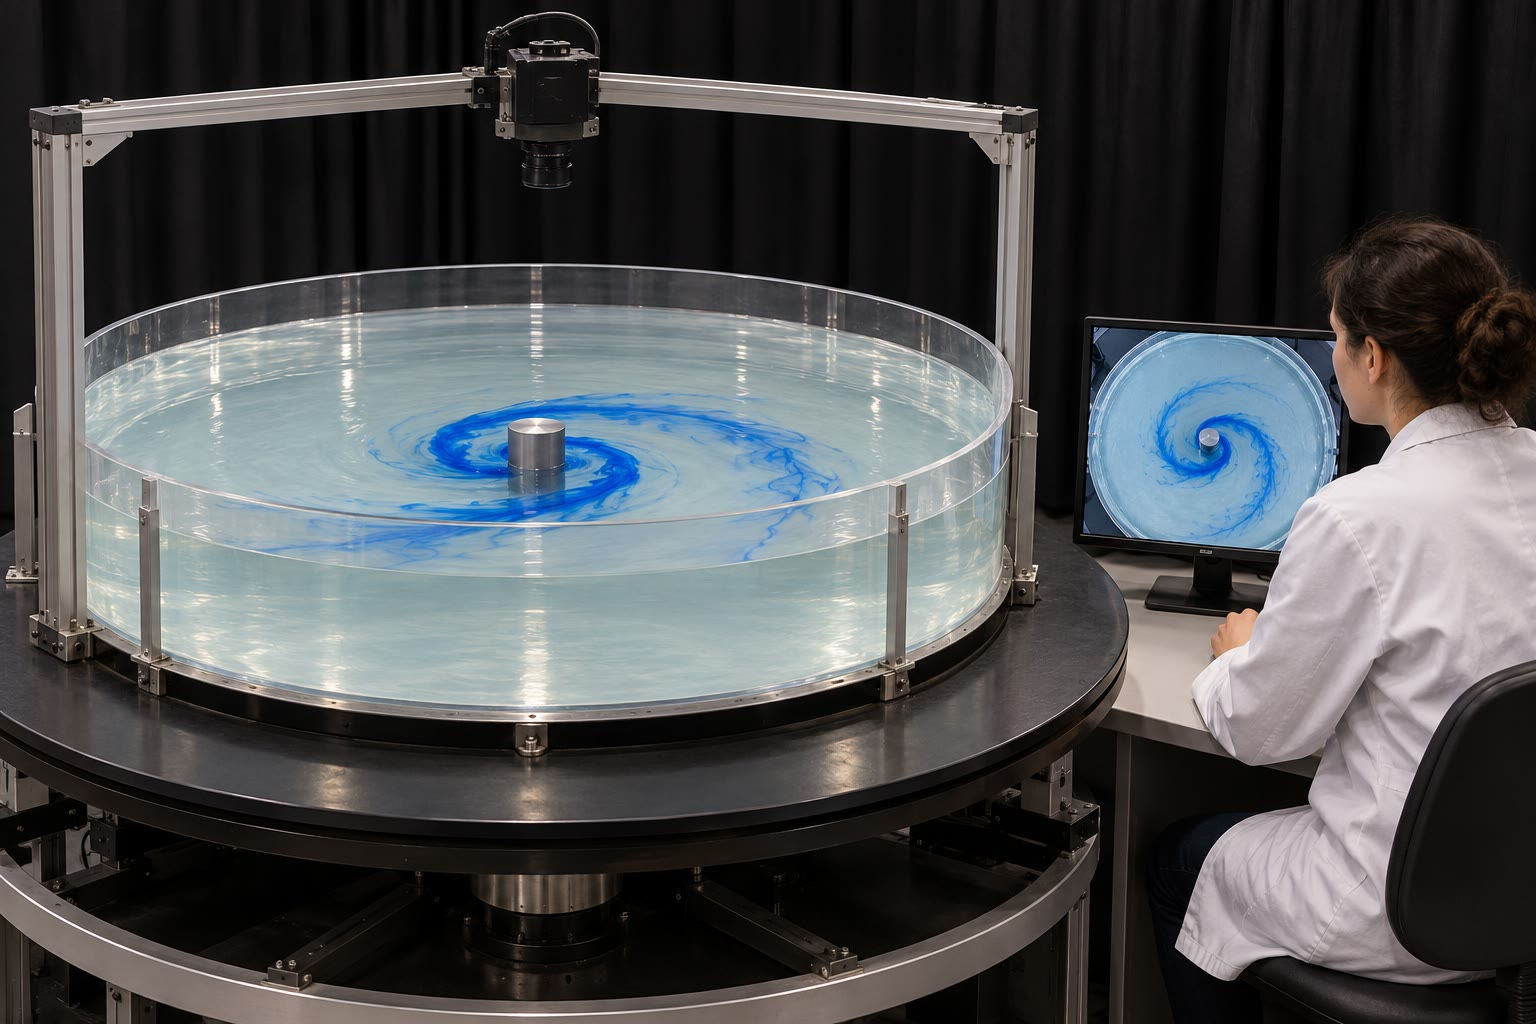
\includegraphics[width=\linewidth]{images/book5/ai/b3-rotating-tank.jpg}

{\scriptsize A rotating tank: dye spiralling round a cylinder, filmed by a
camera that turns with the table (AI-generated illustration).}
\end{minipage}
\end{inthelab}

\section{Exercises}

\begin{exercise}[$\star$]\label{exo:b3:gfd-foundations:1}
Take $\Omega = \qty{7.292115e-5}{rad/s}$. (a)~Compute the Coriolis
parameter and the inertial period at \ang{30}, \ang{45} and \ang{60} N.
(b)~Compute the radius of the inertial circle of a current of
\qty{0.20}{m/s} at the same latitudes. (c)~Compare the inertial period at
\ang{30} with the sidereal day, \qty{23.9345}{h}.
\end{exercise}

\begin{exercise}[$\star$]\label{exo:b3:gfd-foundations:2}
At \ang{45} N, compute the \omterm{def:b3:gfd-foundations:numbers}{Rossby number} of a dust devil (\qty{10}{m/s},
\qty{10}{m}), a sea breeze (\qty{5}{m/s}, \qty{20}{km}), a depression
(\qty{15}{m/s}, \qty{1000}{km}) and an ocean gyre (\qty{0.05}{m/s},
\qty{2000}{km}). Which of them are close to geostrophic balance?
\end{exercise}

\begin{exercise}[$\star$]\label{exo:b3:gfd-foundations:3}
At \ang{45} N the mean temperature of the troposphere, \qty{250}{K}, falls
northward by \qty{5}{K} per \qty{1000}{km}. Using the first term of the
\omterm{thm:b3:gfd-foundations:thermal-wind}{thermal wind} in height, compute the vertical shear of the westerly wind and
the increase of the wind over \qty{10}{km}.
\end{exercise}

\begin{exercise}[$\star$]\label{exo:b3:gfd-foundations:4}
The stability $E = -(1/\rho)\,\mathrm d\rho_\theta/\mathrm dz$ of the upper
kilometre of the ocean lies between \num{50e-8} and \qty{1000e-8}{m^{-1}};
in deep trenches it is \qty{e-8}{m^{-1}}. Compute $N = \sqrt{gE}$, the
period of the buoyancy oscillation and $N$ in cycles per hour for these
three values.
\end{exercise}

\begin{exercise}[$\star\star$]\label{exo:b3:gfd-foundations:5}
A weather system has $U = \qty{10}{m/s}$, $L = \qty{1000}{km}$, $H =
\qty{10}{km}$, at \ang{45} N. (a)~Estimate its vertical velocity and its
vertical acceleration, and compare the latter with $g$ and with the
vertical gradient of the pressure perturbation, $fUL/H$. (b)~Compute the
dropped Coriolis term $\tilde fu$ and compare it with $g$.
\end{exercise}

\begin{exercise}[$\star\star$]\label{exo:b3:gfd-foundations:6}
Take $f = \qty{e-4}{s^{-1}}$ and circular isobars of radius
\qty{300}{km}. (a)~The pressure gradient round a low gives $V_g =
\qty{20}{m/s}$: compute the \omterm{def:b3:gfd-foundations:gradient}{gradient wind}. (b)~Round a high,
$V_g = \qty{5}{m/s}$: compute the \omterm{def:b3:gfd-foundations:gradient}{gradient wind}. (c)~What is the largest
$V_g$ possible round the high, and the wind then?
\end{exercise}

\begin{exercise}[$\star\star$]\label{exo:b3:gfd-foundations:7}
A tank \qty{20}{cm} deep turns once every \qty{6}{s}; its water has $\nu =
\qty{e-6}{m^2/s}$. (a)~Compute $f = 2\Omega$, then the \omterm{def:b3:gfd-foundations:numbers}{Rossby number} of a
flow of \qty{1}{cm/s} past a cylinder \qty{5}{cm} across, and the \omterm{def:b3:gfd-foundations:numbers}{Ekman
number} of the tank. Will a \omterm{thm:b3:gfd-foundations:taylor-proudman}{Taylor column} form? (b)~Theory gives a spin-up
time $H/\sqrt{\nu\Omega}$: compute it in minutes and in turns of the table.
\end{exercise}

\begin{exercise}[$\star\star$]\label{exo:b3:gfd-foundations:8}
In the January zonal mean of 1991--2020 the westerly wind is \qty{4.27}{m/s}
at \qty{850}{hPa} and \qty{40.39}{m/s} at \qty{250}{hPa} at \ang{30} N,
\qty{5.99}{m/s} and \qty{23.17}{m/s} at \ang{45} N. With $R =
\qty{286.9}{J.kg^{-1}.K^{-1}}$, compute the meridional gradient of the
layer-mean temperature at both latitudes, and say why the jet is stronger
at \ang{30} N.
\end{exercise}

\begin{exercise}[$\star\star$]\label{exo:b3:gfd-foundations:9}
(a)~Compute the Rossby radius of the troposphere ($N =
\qty{0.0113}{s^{-1}}$, $H = \qty{11}{km}$, \ang{45} N) and of the upper
ocean ($N = \qty{0.00357}{s^{-1}}$, $H = \qty{1000}{m}$, \ang{40.5} N).
(b)~With $a = \qty{6371}{km}$, compute $\beta$ at both latitudes and the
relative change $\beta L_R/f$ of the Coriolis parameter over each radius.
\end{exercise}

\begin{exercise}[$\star\star\star$]\label{exo:b3:gfd-foundations:10}
A parcel of the surface ocean set moving at $U$ is slowed by a linear
friction: $\mathrm du/\mathrm dt = fv - ru$, $\mathrm dv/\mathrm dt = -fu -
rv$. (a)~Solve with $w = u + \mathrm iv$ and describe the path. (b)~The
parcel is also carried by a steady current $u_0$ eastward: give its
position. (c)~At \ang{45} N with $U = \qty{0.2}{m/s}$, $r^{-1} =
\num{4}\text{ days}$ and $u_0 = \qty{0.05}{m/s}$, give its speed relative to the
current after four days and the distance it has drifted.
\end{exercise}

\begin{exercise}[$\star\star\star$]\label{exo:b3:gfd-foundations:11}
Across an ocean front at \ang{40} N the density of the water increases
northward by \qty{1}{kg/m^3} over \qty{100}{km}, through the upper
\qty{1000}{m}; below, the water is uniform and still. With $\rho_0 =
\qty{1025}{kg/m^3}$, compute the vertical shear of the current and the
current at the surface. In which direction does it flow?
\end{exercise}

\begin{exercise}[$\star\star\star$]\label{exo:b3:gfd-foundations:12}
The annual-mean column at \ang{40.5} N, \ang{30.5} W has potential
densities $\sigma_\theta = \rho_\theta - \qty{1000}{kg/m^3}$ of 26.029 at
the surface, 26.697 at \qty{100}{m}, 27.079 at \qty{500}{m} and 27.628 at
\qty{1000}{m}. (a)~Compute $N$ in each of the three layers, in
\unit{s^{-1}} and in cycles per hour. (b)~Which layer is the most stable,
and why? (c)~Compare the values with the range of the upper ocean in
\cref{exo:b3:gfd-foundations:4}.
\end{exercise}
% ledger: geod5:grs80-defining, earth:Trot, stewart:stability, data:b5-ncep-uwnd, data:b5-woa23-atlantic, earth:Rmean

\section{Problem: Winds over the Steppe of Orrin}

\begin{problem}[{Weekend problem --- the rotation, the stratification and
the winds of an invented plain at \ang{48} N}]
\label{pb:b3:gfd-foundations:1}
The Steppe of Orrin is a flat plain at \ang{48} N with a lake, Lake Orrin,
\qty{12}{km} wide, and a small laboratory with a rotating tank. Take
$\Omega = \qty{7.292115e-5}{rad/s}$, $g = \qty{9.81}{m/s^2}$, $R =
\qty{286.9}{J.kg^{-1}.K^{-1}}$ and $c_p = \qty{1004}{J.kg^{-1}.K^{-1}}$.
All values of the steppe, its lake and its winds are invented.

\medskip\noindent\textbf{Part I --- Does rotation matter?}
\begin{enumerate}
\item Compute the Coriolis parameter and the inertial period at Orrin.
\item Compute the \omterm{def:b3:gfd-foundations:numbers}{Rossby number} of five flows: water draining from a bathtub
  (\qty{0.1}{m/s} over \qty{0.3}{m}); the tank of the laboratory, which turns
  once every \qty{10}{s} (with $f = 2\Omega_{\text{tank}}$; \qty{5}{mm/s}
  over \qty{0.2}{m}); the evening breeze off the lake (\qty{5}{m/s},
  \qty{20}{km}); a depression (\qty{15}{m/s}, \qty{1000}{km}); the gyre of an
  ocean basin at the same latitude (\qty{0.05}{m/s}, \qty{2000}{km}).
\item Which of these flows feel the rotation that drives them, and which are
  close to geostrophic?
\item Compute the \omterm{def:b3:gfd-foundations:numbers}{Ekman number} of the tank (\qty{0.2}{m} deep, $\nu =
  \qty{e-6}{m^2/s}$), of the depression (eddy viscosity \qty{10}{m^2/s},
  depth \qty{10}{km}) and of the gyre (eddy viscosity \qty{e-3}{m^2/s},
  depth \qty{1000}{m}).
\item The Ekman layer has the thickness $\delta = \sqrt{2\nu/f}$. Show that
  $\delta/H = \sqrt{2\,\mathrm{Ek}}$ and compute $\delta$ for the tank and for
  the air of the steppe.
\item What do these numbers say about where friction matters?
\end{enumerate}

\medskip\noindent\textbf{Part II --- The wind at the ground.}
\begin{enumerate}[resume]
\item At the ground the pressure is \qty{1012.9}{hPa} and the temperature
  \qty{288.1}{K}. Compute the density of the air.
\item The sea-level pressure falls northward by \qty{4}{hPa} per
  \qty{300}{km}. Compute the geostrophic wind and give its direction.
\item The same gradient surrounds a depression whose isobars have a radius
  of \qty{600}{km}. Compute the \omterm{def:b3:gfd-foundations:numbers}{Rossby number} of the isobars and the
  \omterm{def:b3:gfd-foundations:gradient}{gradient wind}.
\item The same gradient surrounds an anticyclone of the same radius.
  Compute the \omterm{def:b3:gfd-foundations:gradient}{gradient wind}, and the largest pressure gradient, in
  \unit{hPa} per \qty{300}{km}, that the anticyclone can hold.
\end{enumerate}

\medskip\noindent\textbf{Part III --- Stratification.}
\begin{enumerate}[resume]
\item The temperature of the troposphere falls by \qty{6.49}{K/km}.
  Compute the dry adiabatic lapse rate $g/c_p$, and $N$ and the period of
  the buoyancy oscillation at \qty{5}{km}, where the temperature is
  \qty{255.7}{K}.
\item Above \qty{11}{km} the air is isothermal at \qty{216.6}{K}. Show that
  $N^2 = g^2/(c_pT)$ there, and compute $N$ and its ratio to the value of
  question~11.
\item Compute the Rossby radius of the troposphere of Orrin, with the $N$ of
  question~11 and $H = \qty{10}{km}$, and compare it with the size of the
  depression of Part~I.
\item In summer, the upper \qty{20}{m} of Lake Orrin are lighter than the
  deep water by \qty{1.5}{kg/m^3} ($\rho_0 = \qty{1000}{kg/m^3}$). Compute
  the reduced gravity $g' = g\,\Delta\rho/\rho_0$, the speed $\sqrt{g'h}$ of
  the slow internal waves of the upper layer, and the Rossby radius
  $\sqrt{g'h}/f$.
\item Will the rotation of the Earth shape the internal motions of the lake?
\end{enumerate}

\medskip\noindent\textbf{Part IV --- The thermal wind.}
\begin{enumerate}[resume]
\item Two radiosonde stations stand \qty{600}{km} apart on the same
  meridian. The mean temperature of the layer from the ground,
  \qty{1013}{hPa}, to \qty{265}{hPa}, about \qty{10}{km}, is \qty{253.0}{K}
  at the southern station and \qty{249.4}{K} at the northern. Compute the
  meridional temperature gradient in \unit{K} per \qty{1000}{km}.
\item The thickness of a layer between two pressures is $\Delta z = (R\bar
  T/g)\ln(p_b/p_t)$. Compute it at both stations, and the slope of the
  \qty{265}{hPa} surface relative to the ground-level one.
\item Deduce the increase of the geostrophic wind from the ground to
  \qty{265}{hPa}, from that slope.
\item Compute the same increase with the \omterm{thm:b3:gfd-foundations:thermal-wind}{thermal wind} theorem in pressure.
\item Is the air of the steppe \omterm{def:b3:gfd-foundations:baroclinic}{barotropic} or \omterm{def:b3:gfd-foundations:baroclinic}{baroclinic}? What would the wind
  at \qty{265}{hPa} be if it were \omterm{def:b3:gfd-foundations:baroclinic}{barotropic}?
\item Compute the increase from the first term of the \omterm{thm:b3:gfd-foundations:thermal-wind}{thermal wind} in
  height, with the mean temperature of the standard troposphere between 0
  and \qty{10}{km}, \qty{255.7}{K}, and compare.
\item Compute the wind at \qty{541}{hPa}, about \qty{5}{km}, assuming the
  temperature gradient is the same at every level.
\item The Richardson number $N^2/(\partial u/\partial z)^2$ must fall below
  0.25 for the shear to drive turbulence. Compute it for the troposphere of
  Orrin.
\item In January the zonal-mean westerly at \qty{250}{hPa} is \qty{23.2}{m/s}
  at \ang{45} N and \qty{40.4}{m/s} at \ang{30} N. Compare with the wind of
  Orrin, and explain why a local wind can exceed the zonal mean.
\item Give the geostrophic wind at \qty{10}{km} above the Steppe of Orrin.
\end{enumerate}
\end{problem}
% ledger: geod5:grs80-defining, stewart:stability, data:b5-ncep-uwnd, nasa:grc-atmos
